\documentclass[11pt,a4paper,landscape,fontset=fandol]{ctexart}
\usepackage[margin=12mm,headheight=15pt]{geometry}
\usepackage{graphicx}
\usepackage{booktabs}
\usepackage{array}
\usepackage[table]{xcolor}
\usepackage{fancyhdr}
\usepackage{caption}
\usepackage{microtype}

\definecolor{accent}{HTML}{1F5A7A}
\definecolor{light}{HTML}{EAF1F5}
\definecolor{muted}{HTML}{4C5963}
\setlength{\parindent}{0pt}
\setlength{\parskip}{4pt}
\captionsetup{font=small,labelformat=empty,skip=2pt}
\pagestyle{fancy}
\fancyhf{}
\fancyhead[L]{\color{muted}\small 30k / 200k 非结构网格结果汇总}
\fancyhead[R]{\color{muted}\small SI 与 RSI 射线效应对比}
\fancyfoot[C]{\small\thepage}
\renewcommand{\headrulewidth}{0.4pt}

\newcommand{\sectiontitle}[2]{%
  {\color{accent}\LARGE\bfseries #1}\hfill{\large\color{muted}#2}\par
  \vspace{2mm}\color{accent}\hrule\color{black}\vspace{4mm}
}
\newcommand{\imgtwo}[2]{%
  \begin{minipage}[t]{0.485\textwidth}\centering
    \includegraphics[width=\linewidth,height=0.345\textheight,keepaspectratio]{#1}
    \captionof{figure}{#2}
  \end{minipage}
}
\newcommand{\imgthree}[2]{%
  \begin{minipage}[t]{0.315\textwidth}\centering
    \includegraphics[width=\linewidth,height=0.245\textheight,keepaspectratio]{#1}
    \captionof{figure}{#2}
  \end{minipage}
}
\newcommand{\methodnote}{\small\color{muted}粗角度 SI：$S_4$（24 个角度）；细角度 SI、RSI、RSI-tail：$S_{32}$（1088 个角度）；RSI sample 数：512。\color{black}}

\begin{document}
\thispagestyle{empty}
\vspace*{7mm}
{\color{accent}\Huge\bfseries 30k / 200k 非结构网格计算结果}\par
\vspace{3mm}
{\Large SI、RSI 与 RSI-tail 射线效应图像汇总}\par
\vspace{8mm}

\begin{minipage}[t]{0.48\textwidth}
  {\large\bfseries 计算参数}\par\vspace{2mm}
  \rowcolors{2}{light}{white}
  \begin{tabular}{>{\bfseries}p{0.34\linewidth}p{0.58\linewidth}}
    \toprule
    项目 & 设置 \\
    \midrule
    粗角度 SI & $S_4$，角度数量 $M=4(4+2)=24$ \\
    细角度 SI & $S_{32}$，角度数量 $M=32(32+2)=1088$ \\
    RSI / RSI-tail & $S_{32}$，角度数量 1088 \\
    RSI sample 数 & 512 \\
    RSI-tail & 512 samples；额外平均 10 步 \\
    Iso 图取值 & $1,\ 0.5,\ 0.05$ \\
    \bottomrule
  \end{tabular}
\end{minipage}\hfill
\begin{minipage}[t]{0.48\textwidth}
  {\large\bfseries 网格信息}\par\vspace{2mm}
  \rowcolors{2}{light}{white}
  \begin{tabular}{>{\bfseries}p{0.25\linewidth}p{0.31\linewidth}p{0.34\linewidth}}
    \toprule
    标记 & 四面体单元数 & 平均单元体积 \\
    \midrule
    30k & 36,470 & $2.74198\times10^{-5}$ \\
    200k & 164,151 & $6.09195\times10^{-6}$ \\
    \bottomrule
  \end{tabular}
  \vspace{7mm}

  {\large\bfseries 图像说明}\par\vspace{2mm}
  Iso 图展示三个等值面，取值依次为 1、0.5、0.05。截面图包括 $y=0$ 原始结果，以及 $y=0.5$ 上分别截去低于 0.015 和 0.02 数值后的结果。SI coarse 另保留一张未截断的 $y=0.5$ 图作为参照。每种网格还单独给出求解器实际施加入射的底面三角形区域。
\end{minipage}

\vfill
{\color{muted}\small 注：30k 与 200k 为目录中的近似网格标记；表中给出数据文件内的实际四面体单元数。平均体积由对应 cells.csv 的 volume 列计算，两个单位立方体网格的总体积均为 1。}
\clearpage

% -------------------- 30k --------------------
\sectiontitle{30k 网格：实际入射区域}{底面 $y=0$；36,470 cells}
\begin{center}
  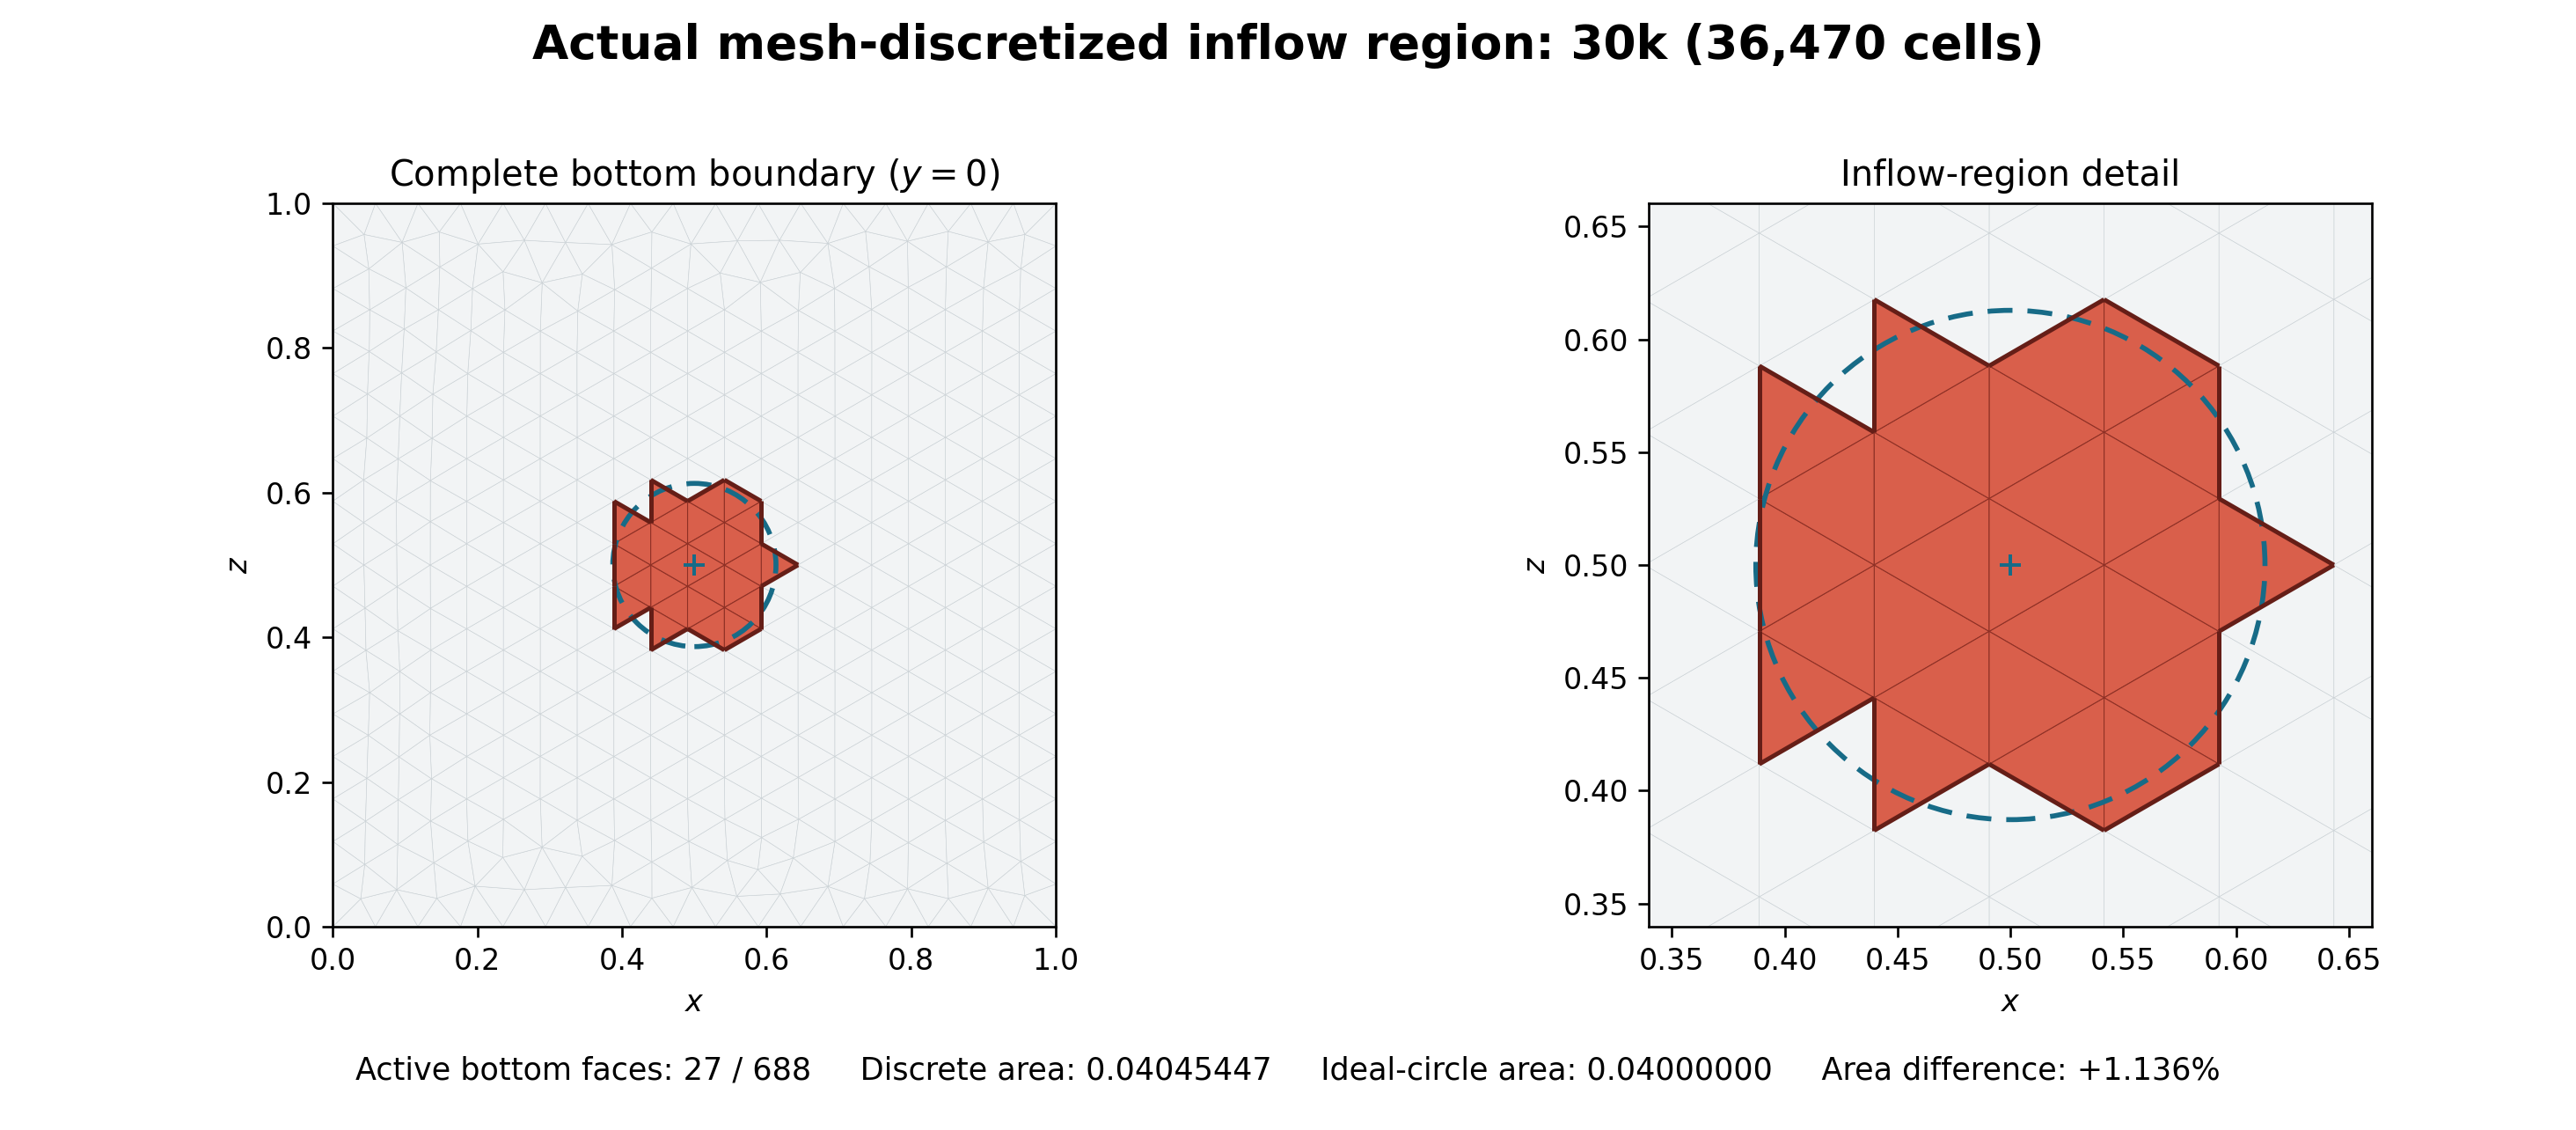
\includegraphics[width=0.95\textwidth,height=0.71\textheight,keepaspectratio]{30k_actual_inflow_region.png}
\end{center}
\vspace{-2mm}
\small
红色区域是求解器真正施加入射的完整三角面并集；蓝色虚线是面积为 0.04 的理想圆（圆心 $(0.5,0.5)$，半径 $0.2/\sqrt{\pi}$），仅用于参照。旧版 \texttt{faces.csv} 不含面积重叠比例，因此采用面中心判定：三角面中心落在理想圆内时，整个三角面均施加入射。30k 底面共有 688 个三角面，其中 27 个被激活；实际离散面积为 0.04045447，比理想圆面积大 1.136\%。
\clearpage

\sectiontitle{30k 网格：Iso 等值面}{36,470 cells；平均体积 $2.74198\times10^{-5}$}
\methodnote\par\vspace{2mm}
\imgtwo{30k_Iso_SI_COARSE.png}{SI coarse：$S_4$，24 个角度；Iso = 1, 0.5, 0.05}\hfill
\imgtwo{30k_Iso_SI_FINE.png}{SI fine：$S_{32}$，1088 个角度；Iso = 1, 0.5, 0.05}\par\vfill
\imgtwo{30k_Iso_RSI.png}{RSI：$S_{32}$，1088 个角度，512 samples；Iso = 1, 0.5, 0.05}\hfill
\imgtwo{30k_Iso_RSI_TAIL.png}{RSI-tail：$S_{32}$，1088 个角度，512 samples；Iso = 1, 0.5, 0.05}
\clearpage

\sectiontitle{30k 网格：$y=0$ 截面}{四种方法对比}
\methodnote\par\vspace{2mm}
\imgtwo{30k_SI_COARSE_y=0.png}{SI coarse，$y=0$}\hfill
\imgtwo{30k_SI_FINE_y=0.png}{SI fine，$y=0$}\par\vfill
\imgtwo{30k_RSI_y=0.png}{RSI，$y=0$，512 samples}\hfill
\imgtwo{30k_RSI_TAIL_y=0.png}{RSI-tail，$y=0$，512 samples}
\clearpage

\sectiontitle{30k 网格：SI 的 $y=0.5$ 截面}{未截断结果及阈值对比}
\methodnote\par\vspace{2mm}
\imgthree{30k_SI_COARSE_y=0.5.png}{SI coarse：未截断}\hfill
\imgthree{30k_SI_COARSE_y=0.5_cut_off_below0.015.png}{SI coarse：截去 $<0.015$}\hfill
\imgthree{30k_SI_COARSE_y=0.5_cut_off_below_0.02.png}{SI coarse：截去 $<0.02$}\par\vfill
\hfill\imgthree{30k_SI_FINE_y=0.5_cut_off_below0.015.png}{SI fine：截去 $<0.015$}\hfill
\imgthree{30k_SI_FINE_y=0.5_cut_off_below0.02.png}{SI fine：截去 $<0.02$}\hfill\mbox{}
\clearpage

\sectiontitle{30k 网格：RSI 的 $y=0.5$ 截面}{阈值对比；512 samples}
\methodnote\par\vspace{2mm}
\imgtwo{30k_RSI_y=0.5_cut_off_below_0.015.png}{RSI：截去 $<0.015$}\hfill
\imgtwo{30k_RSI_y=0.5_cut_off_below_0.02.png}{RSI：截去 $<0.02$}\par\vfill
\imgtwo{30k_RSI_TAIL_y=0.5_cut_off_below_0.015.png}{RSI-tail：截去 $<0.015$}\hfill
\imgtwo{30k_RSI_TAIL_y=0.5_cut_off_below_0.02.png}{RSI-tail：截去 $<0.02$}
\clearpage

% -------------------- 200k --------------------
\sectiontitle{200k 网格：实际入射区域}{底面 $y=0$；164,151 cells}
\begin{center}
  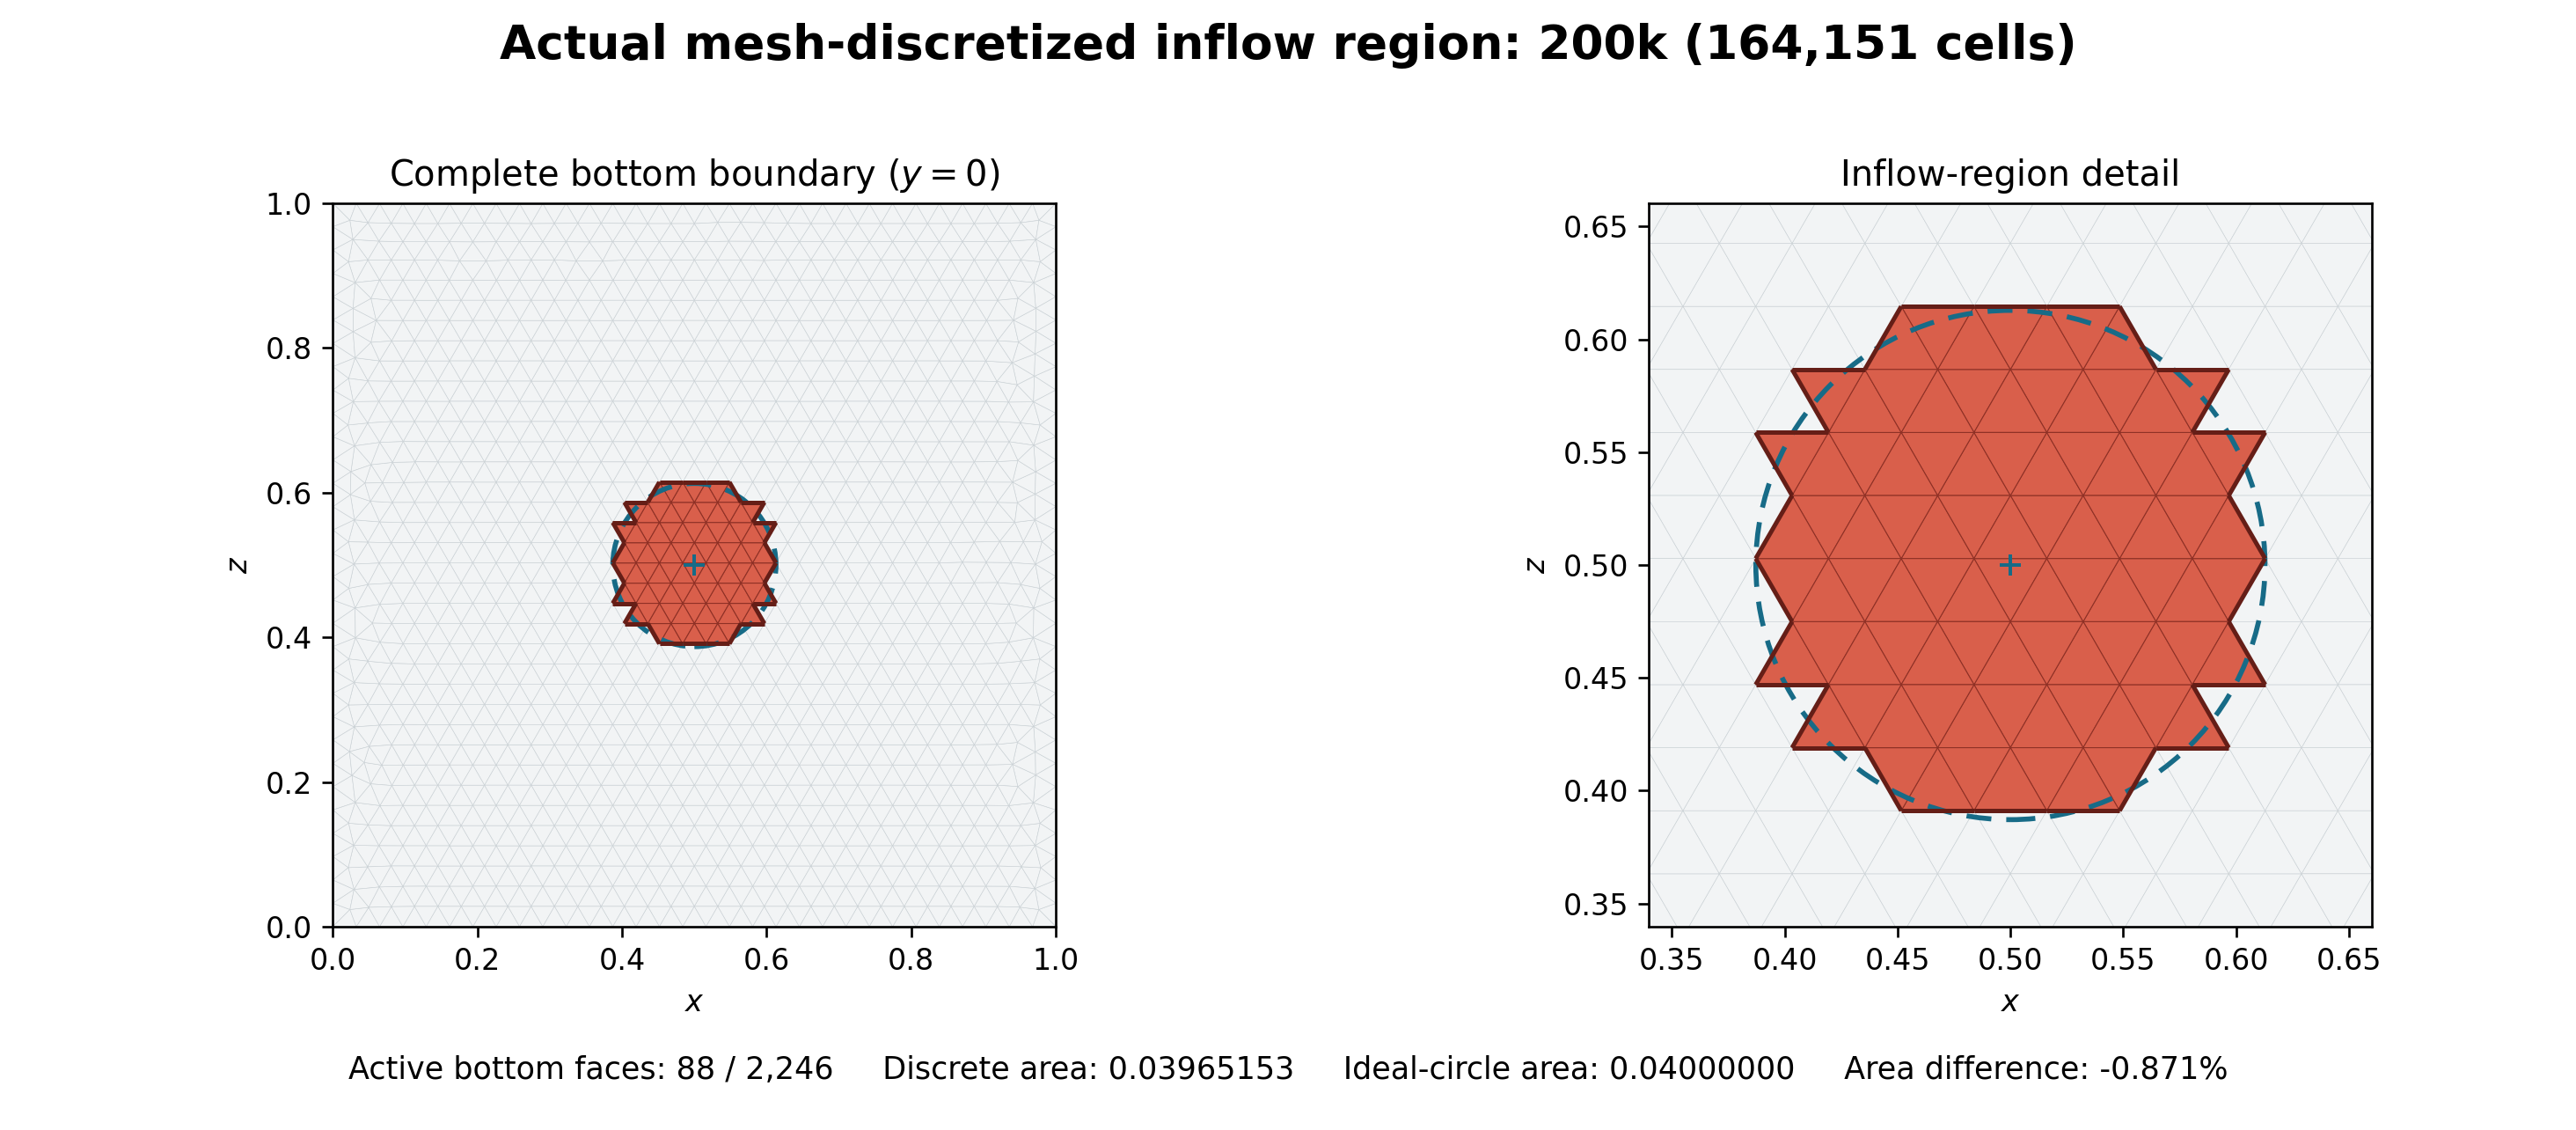
\includegraphics[width=0.95\textwidth,height=0.71\textheight,keepaspectratio]{200k_actual_inflow_region.png}
\end{center}
\vspace{-2mm}
\small
红色区域是求解器真正施加入射的完整三角面并集；蓝色虚线是面积为 0.04 的理想圆（圆心 $(0.5,0.5)$，半径 $0.2/\sqrt{\pi}$），仅用于参照。旧版 \texttt{faces.csv} 不含面积重叠比例，因此采用面中心判定：三角面中心落在理想圆内时，整个三角面均施加入射。200k 底面共有 2,246 个三角面，其中 88 个被激活；实际离散面积为 0.03965153，比理想圆面积小 0.871\%。
\clearpage

\sectiontitle{200k 网格：Iso 等值面}{164,151 cells；平均体积 $6.09195\times10^{-6}$}
\methodnote\par\vspace{2mm}
\imgtwo{200k_Iso_SI_COARSE.png}{SI coarse：$S_4$，24 个角度；Iso = 1, 0.5, 0.05}\hfill
\imgtwo{200k_Iso_SI_FINE.png}{SI fine：$S_{32}$，1088 个角度；Iso = 1, 0.5, 0.05}\par\vfill
\imgtwo{200k_Iso_RSI.png}{RSI：$S_{32}$，1088 个角度，512 samples；Iso = 1, 0.5, 0.05}\hfill
\imgtwo{200k_Iso_RSI_TAIL.png}{RSI-tail：$S_{32}$，1088 个角度，512 samples；Iso = 1, 0.5, 0.05}
\clearpage

\sectiontitle{200k 网格：$y=0$ 截面}{四种方法对比}
\methodnote\par\vspace{2mm}
\imgtwo{200k_SI_COARSE_y=0.png}{SI coarse，$y=0$}\hfill
\imgtwo{200k_SI_FINE_y=0.png}{SI fine，$y=0$}\par\vfill
\imgtwo{200k_RSI_y=0.png}{RSI，$y=0$，512 samples}\hfill
\imgtwo{200k_RSI_TAIL_y=0.png}{RSI-tail，$y=0$，512 samples}
\clearpage

\sectiontitle{200k 网格：SI 的 $y=0.5$ 截面}{未截断结果及阈值对比}
\methodnote\par\vspace{2mm}
\imgthree{200k_SI_COARSE_y=0.5.png}{SI coarse：未截断}\hfill
\imgthree{200k_SI_COARSE_y=0.5_cut_off_below_0.015.png}{SI coarse：截去 $<0.015$}\hfill
\imgthree{200k_SI_COARSE_y=0.5_cut_off_below_0.02.png}{SI coarse：截去 $<0.02$}\par\vfill
\hfill\imgthree{200k_SI_FINE_y=0.5_cut_off_below0.015.png}{SI fine：截去 $<0.015$}\hfill
\imgthree{200k_SI_FINE_y=0.5_cut_off_below0.02.png}{SI fine：截去 $<0.02$}\hfill\mbox{}
\clearpage

\sectiontitle{200k 网格：RSI 的 $y=0.5$ 截面}{阈值对比；512 samples}
\methodnote\par\vspace{2mm}
\imgtwo{200k_RSI_y=0.5_cut_off_below_0.015.png}{RSI：截去 $<0.015$}\hfill
\imgtwo{200k_RSI_y=0.5_cut_off_below_0.02.png}{RSI：截去 $<0.02$}\par\vfill
\imgtwo{200k_RSI_TAIL_y=0.5_cut_off_below_0.015.png}{RSI-tail：截去 $<0.015$}\hfill
\imgtwo{200k_RSI_TAIL_y=0.5_cut_off_below_0.02.png}{RSI-tail：截去 $<0.02$}

\end{document}
